\chapter{The Bayes filter}
\label{ch:bayes}

Every filter in this book is an approximation of one recursion. This
chapter derives it, from the two assumptions of
Chapter~\ref{ch:statespace} and nothing else, and then implements it with
no approximation other than discretisation: on a grid. The grid shows what
the exact belief looks like (sometimes it has two separate bumps) and why
we cannot afford a grid in general.

\section{Belief}

The robot never knows its pose exactly. What it knows is described by a
probability distribution over the possible poses: sharp when it is sure,
spread out when it is not, with several bumps when several places fit what
it has seen. This distribution is what a filter computes.

Three words come back all the time. A distribution of the state held
\emph{before} a measurement is taken into account is called a
\emph{prior}; the distribution \emph{after} it is the \emph{posterior}.
And $p(\z\mid\x)$, read as a function of the state $\x$ for the
measurement $\z$ actually received, is the \emph{likelihood}: it says how
well each possible state explains that measurement.

\paragraph{What the value of a likelihood means.} The number
$p(\z\mid\x)$ is not the probability of receiving $\z$: for a continuous
measurement the probability of any exact value is zero. It is the value of
a density, a probability per unit volume (\cref{sec:shape}). For a small
region $B$ around the reading that was received,
\[
  \Pr(\z\in B\mid\x)\approx p(\z\mid\x)\times\text{volume of }B .
\]
The volume of $B$ is the same whatever the state $\x$. So comparing two
states by their likelihoods is comparing the probabilities that they give
to ``a reading close to the one received'': if
$p(\z\mid\x)=3\,p(\z\mid\x')$, such a reading is three times more
probable from $\x$ than from $\x'$. This is also what a sensor really
delivers, since its resolution is finite: a small cell, not an exact
value.

This is what makes it legitimate to weigh the states by their likelihood,
as Bayes' rule does below, and to prefer the state under which the
measurement is the most likely, the \emph{maximum-likelihood} choice
(used in \cref{sec:ekf-association} to decide which landmark a reading
comes from). Two cautions go with it.
\begin{itemize}[nosep]
  \item The likelihood is a density in $\z$, not in $\x$: read as a
    function of $\x$ it need not integrate to one, and only ratios between
    states have a meaning. Changing the unit of $\z$ multiplies all the
    likelihoods by the same factor and changes no ratio.
  \item It ranks the states by how well they explain the measurement. It
    does not say how probable a state is: that needs a prior as well, and
    is the posterior.
\end{itemize}

\begin{definition}{Belief and predicted belief}{belief}
The \emph{belief} at step $t$ is the posterior distribution of the
current state given everything observed so far,
\[
  \bel(\x_t)=p(\x_t\mid\z_{1:t},\uu_{0:t-1}),
\]
and the \emph{predicted belief} is the distribution of the next state
after the next control but before the next measurement,
\[
  \belbar(\x_{t+1})=p(\x_{t+1}\mid\z_{1:t},\uu_{0:t}).
\]
\end{definition}

The belief is the complete answer to ``where is the robot?''. A filter
may summarise it (by its mean and covariance, say), but every summary
loses information, and some summaries can be badly misleading
(\cref{sec:twobumps}). Before any measurement, the belief is the
distribution of the start pose, $\bel(\x_0)=p(\x_0)$: concentrated around
one pose if the start is known, wide if it is not. (A start that is known
exactly would be a single point, a distribution without a density; in
practice the start is always given a small spread.)

\section{The recursion}

The belief can be computed step by step: the belief at step $t+1$ is
obtained from the belief at step $t$, the control $\uu_t$ and the
measurement $\z_{t+1}$, with no need to go back to older data
(\cref{fig:bayesflow}). Each cycle has two stages: \emph{predict}, which
accounts for the motion, and \emph{update}, which accounts for the
measurement.

\begin{figure}[ht]
\centering
\begin{tikzpicture}[>=Stealth,
  box/.style={draw,thick,rounded corners=2pt,minimum height=9mm,
    minimum width=21mm,font=\small,fill=defblue!8},
  lab/.style={font=\small,align=center}]
  \node[box] (b0) at (0,0) {$\bel(\x_t)$};
  \node[box] (bb) at (6.1,0) {$\belbar(\x_{t+1})$};
  \node[box] (b1) at (12.2,0) {$\bel(\x_{t+1})$};
  \draw[->,thick] (b0) -- (bb) node[pos=0.5,above,lab] {predict}
    node[pos=0.5,below,lab] {control $\uu_t$\\motion model};
  \draw[->,thick] (bb) -- (b1) node[pos=0.5,above,lab] {update}
    node[pos=0.5,below,lab] {measurement $\z_{t+1}$\\likelihood};
  \draw[->,thick,black!50,rounded corners=4pt] (b1.north) -- ++(0,0.7)
    -| (b0.north) node[pos=0.25,above,font=\small,black!60]
    {next cycle: $t\leftarrow t+1$};
\end{tikzpicture}
\caption{One cycle of the Bayes filter. The predict step turns the belief
into the predicted belief, using the control and the motion model. The
update step turns the predicted belief into the new belief, using the
measurement and its likelihood.}
\label{fig:bayesflow}
\end{figure}

When the state takes only a few values, a cycle can be done by hand.

\begin{example}{A two-state filter}{grassgravel}
The robot is either on the grass ($G$) or on the gravel path ($P$). At
each step it stays on the same surface with probability $0.9$. A vibration
sensor says ``rough'' with probability $0.8$ on gravel and $0.3$ on grass.
The current belief is $\bel=(0.8,\,0.2)$ for $(G,P)$: the robot is
probably on the grass.

\emph{Predict.} The robot is on the grass at the next step if it was on
the grass and stayed, or on the path and left it:
$\belbar(G)=0.9\times0.8+0.1\times0.2=0.74$, and
$\belbar(P)=0.1\times0.8+0.9\times0.2=0.26$. The belief has moved towards
$(0.5,0.5)$: it is less sure than before.

\emph{Update.} The sensor says ``rough''. Multiply the predicted
probability of each state by the probability that this state gives the
reading ``rough'', $p(\text{rough}\mid G)=0.3$ and
$p(\text{rough}\mid P)=0.8$: $0.3\times0.74=0.222$ for $G$ and
$0.8\times0.26=0.208$ for $P$.

These two products are not yet the new belief. Each is the probability of
two things together: $0.222$ is the probability that the robot is on the
grass \emph{and} the sensor says ``rough'' (probability $0.74$ to be on
the grass, then $0.3$ that the grass gives ``rough''), and $0.208$ the
probability that it is on the path \emph{and} the sensor says ``rough''.
These are the only two ways of getting the reading ``rough'', so their sum
\[
  0.222+0.208=0.43
\]
is the probability of the reading ``rough'' itself, computed from the
predicted belief: the probability that the filter gave to this reading
before seeing it. Before the reading arrives, there are four possible
cases, a surface and a reading, and their probabilities add up to $1$:
\begin{center}
\begin{tabular}{lccc}
  \toprule
  & ``rough'' & ``smooth'' & total\\
  \midrule
  grass ($0.74$) & $0.74\times0.3=0.222$ & $0.74\times0.7=0.518$ & $0.74$\\
  path ($0.26$)  & $0.26\times0.8=0.208$ & $0.26\times0.2=0.052$ & $0.26$\\
  \midrule
  total & $0.43$ & $0.57$ & $1$\\
  \bottomrule
\end{tabular}
\end{center}
The sensor says ``rough'': the column ``smooth'' becomes impossible and is
struck out. Only the two cases of the column ``rough'' remain, and the new
belief is the share of each in their total:
\[
  \bel(G)=\frac{0.222}{0.43}=0.516,\qquad
  \bel(P)=\frac{0.208}{0.43}=0.484 .
\]
Dividing by $0.43$ is what makes the two new probabilities add up to $1$;
it does not change their ratio, which the products already fixed. One
rough reading has almost cancelled the initial confidence in the grass.
(The sum is the rule of total probability, and the division is Bayes'
rule, both recalled below.)
\end{example}

The general recursion is the same computation, with integrals over the
state in place of the sums over two values. Its derivation uses two rules
of probability, recalled here for densities.
\begin{itemize}[nosep]
  \item \emph{Total probability}: $p(a)=\int p(a\mid b)\,p(b)\,\mathrm db$.
    To find how likely $a$ is, go through every possible $b$.
  \item \emph{Bayes' rule}: $p(b\mid a)=p(a\mid b)\,p(b)/p(a)$. It turns
    ``how likely is this observation if the state is $b$'' into ``how
    likely is the state $b$ given this observation''.
\end{itemize}
Both remain true when every term is conditioned on the same extra
variables, which is how they are used below.

\begin{theorem}{Bayes filter}{bayes}
Under \ref{A1}--\ref{A2}, with controls fixed in advance or computed from
the measurements (the two cases of \cref{prop:joint}),
\begin{align}
  \belbar(\x_{t+1})&=\int p(\x_{t+1}\mid\x_t,\uu_t)\,\bel(\x_t)\,
  \mathrm d\x_t, \label{eq:predict}\\
  \bel(\x_{t+1})&=\eta_{t+1}\,p(\z_{t+1}\mid\x_{t+1})\,
  \belbar(\x_{t+1}),\qquad
  \eta_{t+1}^{-1}=\int p(\z_{t+1}\mid\x)\,\belbar(\x)\,\mathrm d\x.
  \label{eq:update}
\end{align}
\end{theorem}

\begin{proof}
Recall what the two beliefs are (\cref{def:belief}):
$\bel(\x_t)=p(\x_t\mid\z_{1:t},\uu_{0:t-1})$, the pose given all the data
up to step $t$, and $\belbar(\x_{t+1})=p(\x_{t+1}\mid\z_{1:t},\uu_{0:t})$,
the next pose given the same data and the control $\uu_t$. The proof
follows \cref{ex:grassgravel} step by step, with integrals in place of
sums.

\emph{Predict, step 1: go through every current pose.} The robot reaches
$\x_{t+1}$ from some current pose $\x_t$. The law of total probability,
with everything conditioned on the data $(\z_{1:t},\uu_{0:t})$, adds up
the ways of reaching $\x_{t+1}$, one for each $\x_t$:
\[
  \underbrace{p(\x_{t+1}\mid\z_{1:t},\uu_{0:t})}_{\belbar(\x_{t+1})}
  =\int p(\x_{t+1}\mid\x_t,\z_{1:t},\uu_{0:t})\;
  p(\x_t\mid\z_{1:t},\uu_{0:t})\,\mathrm d\x_t .
\]
In the example this was $\belbar(G)=0.9\times0.8+0.1\times0.2$: the
probability of moving to $G$ from each state, times the probability of
that state.

\emph{Predict, step 2: the first factor is the motion model.} \ref{A1}
removes everything but $\x_t$ and $\uu_t$: it says that, given $\x_t$ and
$\uu_t$, the next pose is independent of all the earlier variables
together, hence also of those that appear here, $\z_{1:t}$ and
$\uu_{0:t-1}$. This includes the last measurement $\z_t$: the next pose
is $f(\x_t,\uu_t+\bepsilon_t)$, in which no measurement appears. A
measurement can act on the motion only through the control, when the
control is computed from it, and the control $\uu_t$ is given. So the
first factor is $p(\x_{t+1}\mid\x_t,\uu_t)$.

\emph{Predict, step 3: the second factor is the belief.} The control
$\uu_t$ carries no information about $\x_t$ beyond what is already given
(it is fixed in advance, or computed from the measurements $\z_{1:t}$),
so it can be dropped, which leaves
$p(\x_t\mid\z_{1:t},\uu_{0:t-1})=\bel(\x_t)$ (\cref{sec:bayesnet-mower},
statement~(c), checks this independence on the graph of the model).
Substituting both factors gives \eqref{eq:predict}.

\emph{Update, step 1: Bayes' rule.} Now the measurement $\z_{t+1}$
arrives. Bayes' rule, with everything conditioned on the data
$(\z_{1:t},\uu_{0:t})$ already in hand, gives
\[
  \underbrace{p(\x_{t+1}\mid\z_{1:t+1},\uu_{0:t})}_{\bel(\x_{t+1})}=
  \frac{p(\z_{t+1}\mid\x_{t+1},\z_{1:t},\uu_{0:t})\;
  p(\x_{t+1}\mid\z_{1:t},\uu_{0:t})}
  {p(\z_{t+1}\mid\z_{1:t},\uu_{0:t})}.
\]
(Bayes' rule itself comes from writing the probability of $\x_{t+1}$ and
$\z_{t+1}$ together in two ways: $p(\x_{t+1}\mid\z_{t+1})\,p(\z_{t+1})=
p(\z_{t+1}\mid\x_{t+1})\,p(\x_{t+1})$, all conditioned on the data, and
dividing by $p(\z_{t+1})$.)

\emph{Update, step 2: the numerator.} \ref{A2} reduces its first factor
to $p(\z_{t+1}\mid\x_{t+1})$ (given $\x_{t+1}$, the measurement is
independent of all the earlier variables, hence of $\z_{1:t}$ and
$\uu_{0:t}$), and its second factor is $\belbar(\x_{t+1})$. The numerator
is therefore $p(\z_{t+1}\mid\x_{t+1})\,\belbar(\x_{t+1})$: the probability
of being at $\x_{t+1}$ \emph{and} receiving the reading $\z_{t+1}$, the
products $0.222$ and $0.208$ of the example.

\emph{Update, step 3: the denominator.} It is the probability of the
reading $\z_{t+1}$ given the data, before knowing where the robot is: the
$0.43$ of the example. It is computed like $0.43=0.222+0.208$, by going
through every possible next pose (total probability again, then \ref{A2}
in the first factor):
\[
  p(\z_{t+1}\mid\z_{1:t},\uu_{0:t})
  =\int p(\z_{t+1}\mid\x,\z_{1:t},\uu_{0:t})\,
   p(\x\mid\z_{1:t},\uu_{0:t})\,\mathrm d\x
  =\int p(\z_{t+1}\mid\x)\,\belbar(\x)\,\mathrm d\x ,
\]
the integral of the numerator over all the poses. This is
$\eta_{t+1}^{-1}$, and the three steps together give \eqref{eq:update}.

\emph{A check.} The denominator does not depend on $\x_{t+1}$, and
dividing by it is exactly what makes the new belief integrate to one:
integrating \eqref{eq:update} over $\x_{t+1}$ gives
$\eta_{t+1}\int p(\z_{t+1}\mid\x)\,\belbar(\x)\,\mathrm d\x=1$. As in the
example, the division fixes the total, not the shape: the shape of the
new belief is set by the numerator alone. This is why the denominator is
often called a \emph{normalising constant}.
\end{proof}

\paragraph{What is a density in these formulas, and what is not.} The
beliefs $\bel$ and $\belbar$ and the likelihood $p(\z\mid\x)$ are
densities: functions that can be evaluated and integrated (the initial
belief $p(\x_0)$ is assumed to have one). The transition
$p(\x_{t+1}\mid\x_t,\uu_t)$ is a distribution \emph{without} a density
(\cref{prop:degenerate}), so \eqref{eq:predict} cannot be read as the
integral of a product of two functions. Here is how it is read instead, in
three steps.

\emph{What \eqref{eq:predict} means.} Go through every current pose
$\x_t$, weighted by its belief $\bel(\x_t)$, and spread it over the poses
it can move to with the control $\uu_t$; $\belbar$ collects all these
spreads. The trouble is only in the spread of one pose: it lies on a thin
surface (\cref{fig:transition}), so it has no density to multiply by
$\bel(\x_t)$.

\emph{The same thing as a recipe.} The spread of one pose $\x$ is the set
of poses $f(\x,\uu_t+\bepsilon)$ for all the possible control noises
$\bepsilon$, weighted by the density of the noise. So a predicted pose is
produced in three moves: draw a current pose $\x$ from $\bel$, draw a
noise $\bepsilon$ from $\Normal(\vect0,M)$, independently, and compute
$f(\x,\uu_t+\bepsilon)$. $\belbar$ is the distribution of the poses
produced this way. The recipe uses only $\bel$, the noise density and the
function $f$, which all exist.

\emph{The same thing as a formula.} A distribution is known once the
average under it of every function $g$ of the pose is known (as in
\cref{sec:assumptions}: $g(\x)=\x$ gives the mean, and the indicator of a
region, $1$ inside and $0$ outside, gives the probability of the region).\footnote{This
view of a distribution, through the averages it gives to functions, is
developed in the companion book (Section~20.7 there), with the
distributions of L.~Schwartz and the $\delta$ notation in which
\eqref{eq:predict} is often written.}
The average of $g$ over the predicted pose can be computed in two ways.
With the density $\belbar$, it is $\int g(\x)\,\belbar(\x)\,\mathrm d\x$.
With the recipe, the predicted pose is $f(\x,\uu_t+\bepsilon)$, where the
pair $(\x,\bepsilon)$ has the density $\bel(\x)\,\rho(\bepsilon)$ (a
product, since the two are drawn independently; $\rho$ is the Gaussian
density of the noise). The two must agree:
\begin{equation}\label{eq:predictnoise}
  \int g(\x)\,\belbar(\x)\,\mathrm d\x
  =\iint g\bigl(f(\x,\uu_t+\bepsilon)\bigr)\,\bel(\x)\,\rho(\bepsilon)\,
  \mathrm d\x\,\mathrm d\bepsilon .
\end{equation}
Every function in this equation can be evaluated: it is \eqref{eq:predict}
with nothing left to interpret. With $g(\x)=\x$, for instance, it says
that the mean of the predicted pose is the average of
$f(\x,\uu_t+\bepsilon)$ over the current poses and the noises.

This is also how the filters of the next chapters compute the prediction:
they push poses and noises through $f$, as in the recipe, and never
evaluate the transition. \Cref{sec:shape} explains why $\belbar$ has a
density when $\bel$ has one. The update \eqref{eq:update} involves
densities only.

\begin{inwords}
\emph{Predict}: push the belief through the motion model. Every possible
current pose spreads into the poses it could move to, weighted by how
likely it was. The belief blurs. \emph{Update}: reweight every pose by how
well it explains what was just seen, then renormalise. The belief
sharpens. Repeat.
\end{inwords}

\Cref{fig:bayescycle} shows one cycle on a one-dimensional example, where
everything can be computed exactly.

\begin{figure}[ht]
\centering
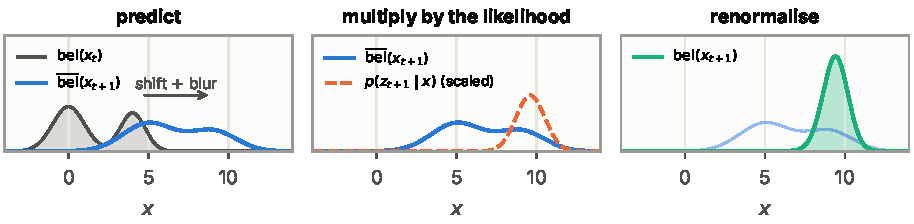
\includegraphics[width=\linewidth]{figures/ch02_bayes_cycle.pdf}
\caption{One cycle of the Bayes filter, computed exactly on a fine 1-D
grid. Predict: a two-bump belief is shifted by the commanded displacement
and blurred by the motion noise. Update: the prediction is multiplied by
the likelihood of the new measurement (dashed) and renormalised. The bump
that agrees with the measurement survives; the other one almost
disappears.}
\label{fig:bayescycle}
\end{figure}


The normaliser has a meaning of its own, which the particle filter will
use in \cref{sec:amcl}.

\begin{proposition}{The normaliser is the predictive likelihood}{evidence}
$\eta_{t+1}^{-1}=p(\z_{t+1}\mid\z_{1:t},\uu_{0:t})$, the value of the
density that the filter assigned to the measurement before seeing it.
For controls fixed in advance, the whole sequence of measurements has the
density
\[
  \log p(\z_{1:T}\mid\uu_{0:T-1})=-\sum_{t=1}^T\log\eta_t ,
\]
and when the controls are computed from the measurements the same sum is
$\log p(\z_{1:T})$.
\end{proposition}

\begin{proof}
\emph{The first claim.} It was obtained in the proof of \cref{thm:bayes}
(update, step~3): the denominator of Bayes' rule is
$p(\z_{t+1}\mid\z_{1:t},\uu_{0:t})$, and it equals
$\int p(\z_{t+1}\mid\x)\,\belbar(\x)\,\mathrm d\x=\eta_{t+1}^{-1}$. With
the index shifted by one, for every $t\ge1$,
\begin{equation}\label{eq:etat}
  \eta_t^{-1}=p(\z_t\mid\z_{1:t-1},\uu_{0:t-1}),
\end{equation}
the density of the measurement $\z_t$ given everything the filter had
before it: the earlier measurements and the controls already applied
(for $t=1$, $\z_{1:0}$ is empty).

\emph{Controls fixed in advance, step 1: the chain rule.} The density of
all the measurements together, given all the controls, is a product of
one factor per measurement, each conditioned on the measurements before
it (the chain rule, $p(a,b)=p(a)\,p(b\mid a)$ applied repeatedly):
\begin{align*}
  p(\z_{1:T}\mid\uu_{0:T-1})
  &=p(\z_1\mid\uu_{0:T-1})\,p(\z_2\mid\z_1,\uu_{0:T-1})\cdots
   p(\z_T\mid\z_{1:T-1},\uu_{0:T-1})\\
  &=\prod_{t=1}^Tp(\z_t\mid\z_{1:t-1},\uu_{0:T-1}).
\end{align*}

\emph{Step 2: compare each factor with \eqref{eq:etat}.} The factor of
$\z_t$ is conditioned on all the controls, $\uu_{0:T-1}$; \eqref{eq:etat}
only on those applied before $\z_t$, $\uu_{0:t-1}$. The difference is the
later controls $\uu_t,\dots,\uu_{T-1}$, and the factors are equal if
these carry no information about $\z_t$ given the rest, that is if
\[
  \z_t\indep\uu_{t:T-1}\mid\z_{1:t-1},\uu_{0:t-1}.
\]
That they are applied after $\z_t$ is not a reason: a conditional density
is about information, not influence (the trap of \cref{sec:assumptions}),
and a later control computed from $\z_t$ would carry information about
it. The reason is the graph of the model (\cref{fig:bayesnet}), read with
the d-separation rule (\cref{def:dsep}). Take a later control $\uu_s$,
$s\ge t$. Fixed in advance, it has no parent, and its only arrow is
$\uu_s\rightarrow\x_{s+1}$. So a path from $\uu_s$ to $\z_t$ starts
$\uu_s\rightarrow\x_{s+1}$, and from $\x_{s+1}$ it must go on along
another arrow: to $\z_{s+1}$ or $\x_{s+2}$, which lead only further into
the future and never back to $\z_t$, or to $\x_s$, along
$\x_{s+1}\leftarrow\x_s$. On every path that reaches $\z_t$, the node
$\x_{s+1}$ therefore has two arrows pointing into it,
$\uu_s\rightarrow\x_{s+1}\leftarrow\x_s$: it is a collider. A collider
blocks the path unless it, or one of its descendants, is given. The
descendants of $\x_{s+1}$ are the later poses and their measurements
$\z_{s+1},\z_{s+2},\dots$, all after $\z_t$; the given variables,
$\z_{1:t-1}$ and $\uu_{0:t-1}$, contain none of them, nor $\x_{s+1}$.
So every path is blocked, and \cref{thm:dsep} gives the independence.

\emph{Step 3: conclude.} Each factor is therefore
$p(\z_t\mid\z_{1:t-1},\uu_{0:t-1})=\eta_t^{-1}$, so
$p(\z_{1:T}\mid\uu_{0:T-1})=\prod_{t=1}^T\eta_t^{-1}$, and taking the
logarithm turns the product into the sum
$-\sum_{t=1}^T\log\eta_t$.

\emph{Controls computed from the measurements.} Now the controls are not
given in advance: $\uu_t=\pi_t(\z_{1:t})$, and the model is the joint
distribution $p(\x_{0:T},\z_{1:T})$ of \cref{prop:joint}(ii). Apply the
chain rule to $p(\z_{1:T})$ itself:
$p(\z_{1:T})=\prod_{t=1}^Tp(\z_t\mid\z_{1:t-1})$. In the factor of $\z_t$
the controls $\uu_0,\dots,\uu_{t-1}$ do not appear, but they are known:
each $\uu_s=\pi_s(\z_{1:s})$, $s\le t-1$, is computed from the
measurements $\z_{1:t-1}$ that are given. Adding to the condition a
variable that is a function of what is already given adds no
information, so
$p(\z_t\mid\z_{1:t-1})=p(\z_t\mid\z_{1:t-1},\uu_{0:t-1})=\eta_t^{-1}$,
and the same sum is $\log p(\z_{1:T})$.
\end{proof}

\begin{inwords}
The proposition gives the filter a measure of its own surprise, which it
computes anyway, since $\eta_t$ is the normaliser of every update.
$\eta_t^{-1}$ is the density that the filter, \emph{before} $\z_t$
arrived, gave to the value that then arrived: the $0.43$ of
\cref{ex:grassgravel}. A value as large as usual means the reading was
about as expected; a much smaller one means the filter had considered it
unlikely. One small value can be bad luck. A run of them cannot be
explained that way: by the second part of the proposition, the product of
the $\eta_t^{-1}$ over a stretch of time is the density that the model
gives to that whole stretch of readings, and a run of small factors makes
it tiny. The model then no longer explains the data: for example the
robot has been picked up and moved. \Cref{sec:amcl} uses exactly this
test to detect such a kidnapping, comparing a short-term average of
$\eta_t^{-1}$ with a long-term one.
\end{inwords}

\section{The grid filter}
\label{sec:grid}

Neither integral of \cref{thm:bayes} has a closed form in general. The
most direct approximation replaces the state space by a finite grid. To
keep the grid two-dimensional, the robot is given a compass
(\cref{sec:sensors}). The compass is accurate ($\sigma_c=0.02$\,rad, about
$1^\circ$), so the heading is taken from its reading and treated as known,
and only the position is uncertain. The state is then the position
$\p_t$ alone.

\begin{definition}{Grid belief}{grid}
Partition the lawn into $n$ square cells $C_1,\dots,C_n$, with centres
$\vect{c}_1,\dots,\vect{c}_n$. The \emph{grid belief} is the vector
$b_i\approx\Pr(\p_t\in C_i\mid\z_{1:t},\uu_{0:t-1})$, with $\sum_ib_i=1$.
\end{definition}

The \emph{convolution} of two functions on the plane is
\[
  (a\ast g)(\p)=\int a(\p-\vect q)\,g(\vect q)\,\mathrm d\vect q .
\]
\begin{figure}[t]
\centering
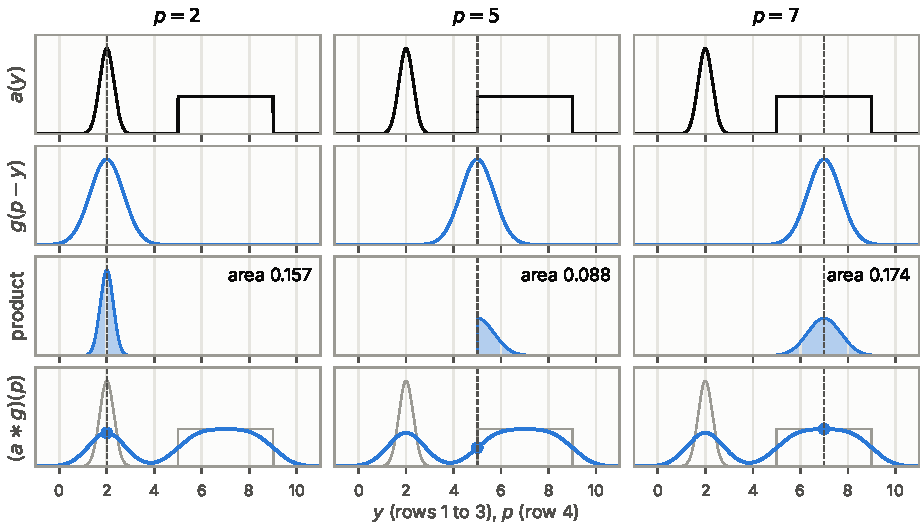
\includegraphics[width=\linewidth]{figures/ch02_conv_read.pdf}
\caption{Computing $a\ast g$ on the line, with $g=\Normal(0,0.7^2)$ and a
function $a$ made of a peak and a plateau (row~1). Each column is one
point $p$ (dashed line). Row~2: the weight $g(p-y)$ given to each value
$a(y)$, centred at $p$. Row~3: the product of the two, whose area is
$(a\ast g)(p)$. Row~4: $a\ast g$ at every $p$ (blue) over $a$ (grey); the
dot is the value of the column. At $p=2$ the peak is lowered ($0.157$ against $0.399$); at $p=5$, where the plateau starts, half of the weight
falls on it, and the value is half its height ($0.088$ against
$0.175$); at $p=7$, in the middle of the plateau, the value is its height
($0.174$).}
\label{fig:convread}
\end{figure}
\emph{How to read it.} To get the value at the point $\p$, look at the
value of $a$ at every point $\p-\vect q$, that is at the offset $\vect q$
from $\p$; weight it by $g(\vect q)$; add up over all the offsets. When
$g$ is a probability density ($g\ge0$, integral $1$), the weights are
non-negative and add up to $1$, so $(a\ast g)(\p)$ is a \emph{weighted
average of the values of $a$ around $\p$}. \Cref{fig:convread} does this
on the line, for three points and then for all of them. When $g$ is concentrated
around $\vect0$, only the values at small offsets count, and $a\ast g$
is a blurred copy of $a$: a sharp peak of $a$ is spread over the region
where $g$ is not small, and a flat region of $a$ is left unchanged
(\cref{fig:convread}, row~4).

\emph{An example.} In one dimension, let $g$ be uniform on $[-h,h]$,
with density $1/(2h)$ there. Then
$(a\ast g)(p)=\frac1{2h}\int_{-h}^{h}a(p-q)\,\mathrm dq$ is the plain
average of $a$ over the interval $[p-h,p+h]$: a \emph{centred} moving
average.\footnote{In time series, a moving average usually uses only past
values, $g(q)=0$ for $q<0$, because the future has not arrived yet; it
then lags behind the signal. Here the variable is a position on the
lawn, which has no past and no future, so a symmetric $g$, which weighs
both sides of $p$ alike, is the natural choice. In time, the Bayes filter
is causal: the belief at time $t$ uses only the measurements up to $t$.}
A Gaussian $g$ gives a centred moving average whose weights fall off with the
distance (\cref{fig:convread}, row~2), as in the predict panel of \cref{fig:bayescycle}.

\emph{The probabilistic meaning.} If $a$ is the density of a random
vector $X$ and $g$ that of an independent $W$, then $a\ast g$ is the
density of the sum $X+W$ (\cref{fig:convresult}). To see it, recall what
a density is: a function $f$ is the density of a random vector $S$ when
$\Pr(S\in B)=\int_Bf(\p)\,\mathrm d\p$ for every region $B$ of the plane.
So we compute $\Pr(X+W\in B)$, in three steps. Write $\mathbf 1_B(\p)$
for $1$ if $\p\in B$ and $0$ otherwise.

\emph{Step 1: the pair.} Because $X$ and $W$ are independent, the pair
$(X,W)$ has the density $a(\vect x)\,g(\vect w)$, the product of their
densities. The probability of an event is the expectation of its
indicator, so
\[
  \Pr(X+W\in B)=\E\bigl[\mathbf 1_B(X+W)\bigr]
  =\int\Bigl(\int\mathbf 1_B(\vect x+\vect w)\,a(\vect x)\,
   \mathrm d\vect x\Bigr)g(\vect w)\,\mathrm d\vect w .
\]

\emph{Step 2: change of variable.} Fix $\vect w$ and look at the inner
integral, over $\vect x$. Put $\p=\vect x+\vect w$, that is
$\vect x=\p-\vect w$. This is a translation, which keeps areas, so
$\mathrm d\vect x=\mathrm d\p$, and
\[
  \int\mathbf 1_B(\vect x+\vect w)\,a(\vect x)\,\mathrm d\vect x
  =\int\mathbf 1_B(\p)\,a(\p-\vect w)\,\mathrm d\p .
\]

\emph{Step 3: swap the two integrals.} Put Step~2 back into Step~1 and
go line by line; the reason for each line is given on its right.%
% the footnote texts are set here, before the display, so that they land
% on the same page as their marks
\addtocounter{footnote}{1}%
\footnotetext{The order of two integrals can be swapped when the
integrand is non-negative (Tonelli's theorem); here it is a product of an
indicator and two densities.}%
\addtocounter{footnote}{1}%
\footnotetext{The integral in brackets is the definition of
$(a\ast g)(\p)$, with the offset called $\vect w$ instead of $\vect q$.}%
\addtocounter{footnote}{-2}%
\begin{align*}
  \Pr(X+W\in B)
  &=\int\Bigl(\int\mathbf 1_B(\p)\,a(\p-\vect w)\,\mathrm d\p\Bigr)
    g(\vect w)\,\mathrm d\vect w
  &&\text{Steps 1 and 2}\\
  &=\int\Bigl(\int\mathbf 1_B(\p)\,a(\p-\vect w)\,g(\vect w)\,
    \mathrm d\p\Bigr)\mathrm d\vect w
  &&\text{$g(\vect w)$ does not depend on $\p$}\\
  &=\int\Bigl(\int\mathbf 1_B(\p)\,a(\p-\vect w)\,g(\vect w)\,
    \mathrm d\vect w\Bigr)\mathrm d\p
  &&\text{swap the order}\footnotemark\\
  &=\int\mathbf 1_B(\p)\Bigl(\int a(\p-\vect w)\,g(\vect w)\,
    \mathrm d\vect w\Bigr)\mathrm d\p
  &&\text{$\mathbf 1_B(\p)$ does not depend on $\vect w$}\\
  &=\int\mathbf 1_B(\p)\,(a\ast g)(\p)\,\mathrm d\p
  &&\text{definition of $a\ast g$}\footnotemark\\
  &=\int_B(a\ast g)(\p)\,\mathrm d\p
  &&\text{$\mathbf 1_B=1$ on $B$, $0$ elsewhere.}
\end{align*}
This holds for every
region $B$, so $a\ast g$ is the density of $X+W$.

Three consequences follow.

\emph{Consequence 1: blurring keeps the total probability.} With $B$ the
whole plane, $\int(a\ast g)(\p)\,\mathrm d\p=\Pr(X+W\in\R^2)=1$.

\emph{Consequence 2: the covariances add.} Write $\tilde X=X-\E X$ and
$\tilde W=W-\E W$ for the centred vectors; their expectations are $\vect0$.
By linearity, $\E[X+W]=\E X+\E W$, so $X+W-\E[X+W]=\tilde X+\tilde W$, and
\begin{align*}
  \Cov(X+W)
  &=\E\bigl[(\tilde X+\tilde W)(\tilde X+\tilde W)\T\bigr]
  &&\text{definition of the covariance}\\
  &=\E[\tilde X\tilde X\T]+\E[\tilde X\tilde W\T]
    +\E[\tilde W\tilde X\T]+\E[\tilde W\tilde W\T]
  &&\text{expand; linearity of }\E\\
  &=\Cov X+\Cov(X,W)+\Cov(X,W)\T+\Cov W .
\end{align*}
The two middle terms are the \emph{cross-covariance} matrix
$\Cov(X,W)=\E[\tilde X\tilde W\T]$ and its transpose. The matrix
$\tilde X\tilde W\T$ is a column times a row, so its entry $(i,j)$ is the
product of the numbers $\tilde X_i$ and $\tilde W_j$ (a number needs no
transpose):
\[
  \tilde X\tilde W\T=
  \begin{pmatrix}\tilde X_1\\ \tilde X_2\end{pmatrix}
  \begin{pmatrix}\tilde W_1&\tilde W_2\end{pmatrix}
  =\begin{pmatrix}\tilde X_1\tilde W_1&\tilde X_1\tilde W_2\\
   \tilde X_2\tilde W_1&\tilde X_2\tilde W_2\end{pmatrix}.
\]
So the entry $(i,j)$ of $\Cov(X,W)$, $\E[\tilde X_i\tilde W_j]$, is the
covariance between the $i$-th
coordinate of $X$ and the $j$-th coordinate of $W$. It is not to be
confused with the off-diagonal entries of $\Cov X$, which are covariances
between two coordinates of the \emph{same} vector $X$. For independent
vectors, the expectation of a product is the product of the
expectations, so $\E[\tilde X_i\tilde W_j]=\E[\tilde X_i]\,\E[\tilde
W_j]=0\times0=0$. Hence $\Cov(X,W)=0$, and
\[
  \Cov(X+W)=\Cov X+\Cov W .
\]

\emph{Consequence 3: blurring widens, in every direction.} Take a unit
vector $\vect u$. The coordinate of a random vector $Y$ along $\vect u$ is
the number $\vect u\T Y$, and its variance is
\[
  \Var(\vect u\T Y)=\E\bigl[(\vect u\T\tilde Y)^2\bigr]
  =\E\bigl[\vect u\T\tilde Y\,\tilde Y\T\vect u\bigr]
  =\vect u\T\,\Cov(Y)\,\vect u ,
\]
where $\tilde Y=Y-\E Y$, and $(\vect u\T\tilde Y)^2=(\vect u\T\tilde
Y)(\tilde Y\T\vect u)$ because a number is equal to its transpose. With
$Y=X+W$ and Consequence~2,
\[
  \Var\bigl(\vect u\T(X+W)\bigr)
  =\vect u\T\Cov(X)\,\vect u+\vect u\T\Cov(W)\,\vect u
  =\Var(\vect u\T X)+\Var(\vect u\T W)\ \ge\ \Var(\vect u\T X),
\]
because a variance is never negative. Along every direction, $X+W$ is at
least as spread as $X$, and strictly more as soon as $W$ has some spread
in that direction: this is what ``blurring widens'' means. On the
covariance ellipses of \cref{fig:covsum}, the ellipse of $X+W$ reaches at
least as far as that of $X$ in every direction, because the reach of a
$2\sigma$ ellipse along $\vect u$ is twice the standard deviation along
$\vect u$.\footnote{The $2\sigma$ ellipse of a covariance $P$ centred at
$\vect c$ is the set of the points $\vect x$ with
$(\vect x-\vect c)\T P^{-1}(\vect x-\vect c)\le4$, that is, of the
points $\vect c+2P^{1/2}\vect v$ with $\norm{\vect v}\le1$, where
$P^{1/2}$ is the symmetric square root of $P$. Its reach along $\vect u$
is the largest value of $\vect u\T(2P^{1/2}\vect v)=2(P^{1/2}\vect
u)\T\vect v$ over $\norm{\vect v}\le1$. By the Cauchy--Schwarz
inequality it is $2\norm{P^{1/2}\vect u}=2\sqrt{\vect u\T P\vect u}$,
reached for $\vect v$ along $P^{1/2}\vect u$.}

\emph{Widening does not keep the shape.} In \cref{fig:covsum}a, $X$ has
the standard deviations $3$ and $0.3$ along two perpendicular axes turned
by $30^\circ$: $\Cov X=R\,\mathrm{diag}(9,\,0.09)\,R\T$, with $R$ the
rotation by $30^\circ$. Its ellipse is $3/0.3=10$ times longer than wide.
The noise $W$ is round, $\Cov W=I$, which can also be written $R\,I\,R\T$
because $RR\T=I$. So
\[
  \Cov(X+W)=R\,\mathrm{diag}(9,\,0.09)\,R\T+R\,I\,R\T
  =R\,\mathrm{diag}(10,\,1.09)\,R\T :
\]
the same axes, with the standard deviations $\sqrt{10}\approx3.16$ and
$\sqrt{1.09}\approx1.04$, a ratio of about $3$ instead of $10$. The round
noise adds the same variance $1$ along both axes, which changes the long
axis little and the short one a lot: the ellipse becomes rounder. The
shape is kept only when $\Cov W$ is a multiple $c\Cov X$: then
$\Cov(X+W)=(1+c)\Cov X$, the same ellipse enlarged by $\sqrt{1+c}$
(\cref{fig:covsum}b, with $c=0.5$). And the covariance is only a
summary: the density itself changes shape too, as the peak of
\cref{fig:convread} shows, lowered and spread.

\emph{Finally, the order does not matter.} The change of variable $\vect q'=\p-\vect q$
gives $\int a(\vect q')\,g(\p-\vect q')\,\mathrm d\vect q'$, so
$a\ast g=g\ast a$.

\begin{figure}[t]
\centering
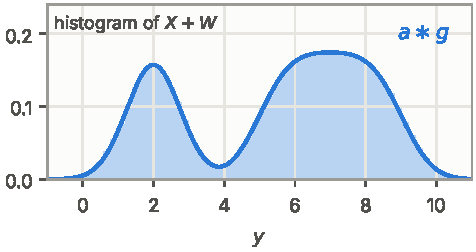
\includegraphics[width=\linewidth]{figures/ch02_conv_result.pdf}
\caption{The density of a sum, on the line. (a) $X$ has the density $a$:
with probability $0.3$ a Gaussian with mean $2$ and standard deviation
$0.3$ (the peak), with probability $0.7$ uniform on $[5,9]$ (the
plateau). (b) $W$, independent of $X$, has the density
$g=\Normal(0,0.7^2)$. (c) The sum $X+W$ has the density $a\ast g$. In
each panel, the histogram is that of $200\,000$ draws, and the curve is
the density.}
\label{fig:convresult}
\end{figure}

\begin{figure}[t]
\centering
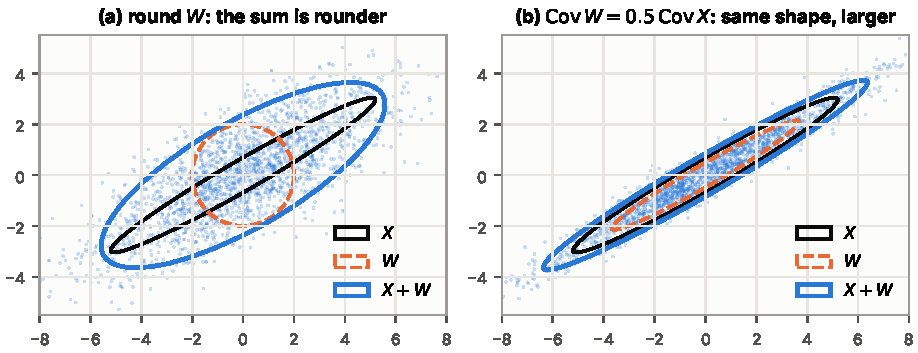
\includegraphics[width=0.85\linewidth]{figures/ch02_cov_sum.pdf}
\caption{The $2\sigma$ covariance ellipses of $X$ (black), of an
independent $W$ (orange, dashed) and of $X+W$ (blue), with $2\,000$
draws of $X+W$. $X$ has the standard deviations $3$ and $0.3$ along axes
turned by $30^\circ$. (a) A round $W$, $\Cov W=I$: the ellipse of $X+W$
contains that of $X$ and is rounder (axis ratio $3.0$ instead of $10$).
(b) $\Cov W=0.5\Cov X$: the ellipse of $X+W$ has the shape of that of
$X$, enlarged by $\sqrt{1.5}\approx1.22$.}
\label{fig:covsum}
\end{figure}

\begin{proposition}[unbreakable]{Prediction with a known heading is a convolution}{conv}
Suppose the heading $\psi_t$ during the drive is known (in the grid
filter, it is the compass reading) and the position moves by
$\p_{t+1}=\p_t+\vect{d}_t+\w_t$, with the displacement
$\vect{d}_t=s_t(\cos\psi_t,\sin\psi_t)$ and a noise
$\w_t\sim\Normal(\vect0,\Sigma_t)$ independent of $\p_t$. Then
\[
  \belbar(\p)=\bigl(\bel(\,\cdot-\vect{d}_t)\ast\Normal(\vect0,\Sigma_t)
  \bigr)(\p),
\]
the belief shifted by $\vect{d}_t$ and blurred by the noise density.
\end{proposition}

\begin{proof}
Write $g$ for the density of $\Normal(\vect0,\Sigma_t)$, and
$\bel(\,\cdot-\vect d_t)$ for the function
$\vect q\mapsto\bel(\vect q-\vect d_t)$: the belief \emph{shifted} by
$\vect d_t$. Its value at $\vect q$ is the old belief at
$\vect q-\vect d_t$, the point from which the displacement $\vect d_t$
leads to $\vect q$. There are two ways to the result. The first gives the
picture, the second checks it on the prediction formula
\eqref{eq:predict}.

\emph{First way: a sum of two independent vectors.} Group the terms as
$\p_{t+1}=(\p_t+\vect d_t)+\w_t$.
\begin{itemize}[nosep]
  \item $\p_t+\vect d_t$ is the old position moved by the known
        displacement, and its density is the shifted belief. For a region
        $B$, write $B-\vect d_t$ for the region $B$ moved by
        $-\vect d_t$. Then
        \[
          \Pr(\p_t+\vect d_t\in B)=\Pr(\p_t\in B-\vect d_t)
          =\int_{B-\vect d_t}\bel(\vect x)\,\mathrm d\vect x
          =\int_B\bel(\vect q-\vect d_t)\,\mathrm d\vect q ,
        \]
        with the change of variable $\vect q=\vect x+\vect d_t$, a
        translation, so $\mathrm d\vect x=\mathrm d\vect q$.
  \item $\w_t$ has the density $g$, and it is independent of $\p_t$,
        hence of $\p_t+\vect d_t$, since $\vect d_t$ is known.
  \item By the probabilistic meaning of the convolution, shown above,
        the sum $\p_{t+1}$ has the density
        $\bel(\,\cdot-\vect d_t)\ast g$.
\end{itemize}

\emph{Second way: from the prediction formula.} Given $\p_t$, the only
random term in $\p_{t+1}=\p_t+\vect d_t+\w_t$ is $\w_t$, and knowing
$\p_t$ does not change its distribution, since the two are independent.
So, given $\p_t$, $\p_{t+1}$ is Gaussian with the mean $\p_t+\vect d_t$
and the covariance $\Sigma_t$. A Gaussian density depends on the point
only through its difference with the mean, so
\[
  p(\p_{t+1}\mid\p_t)=\Normal(\p_{t+1};\,\p_t+\vect d_t,\,\Sigma_t)
  =g(\p_{t+1}-\p_t-\vect d_t).
\]
Call the new position $\p$ and the old one $\vect q$, and go line by
line from \eqref{eq:predict}:
\begin{align*}
  \belbar(\p)
  &=\int g(\p-\vect q-\vect d_t)\,\bel(\vect q)\,\mathrm d\vect q
  &&\text{\eqref{eq:predict} with this transition}\\
  &=\int g(\p-\vect q')\,\bel(\vect q'-\vect d_t)\,\mathrm d\vect q'
  &&\text{$\vect q'=\vect q+\vect d_t$, $\mathrm d\vect q=\mathrm d\vect q'$}\\
  &=\bigl(g\ast\bel(\,\cdot-\vect d_t)\bigr)(\p)
  &&\text{definition of the convolution}\\
  &=\bigl(\bel(\,\cdot-\vect d_t)\ast g\bigr)(\p)
  &&\text{the order does not matter.}
\end{align*}
In the third line, the definition $(a\ast g)(\p)=\int a(\p-\vect q)\,
g(\vect q)\,\mathrm d\vect q$ is used with the roles of the two functions
exchanged: $g$ is evaluated at $\p-\vect q'$, and the shifted belief at
$\vect q'$.
\end{proof}

The same position-only model, with its noise covariance $\Sigma_t$
worked out, is the one the Kalman filter will use in
\cref{sec:linmower}.

On the grid, the prediction of \cref{prop:conv} is done in two moves:
shift the table by $\vect d_t$, then blur it with a discrete Gaussian
filter. A grid cannot represent a blur narrower than a cell. Here the
motion noise has a standard deviation of about $0.4$ units, a tenth of a
cell 4 units wide, so the filter blurs by more than the noise, and the
predicted belief comes out a little wider than the noise warrants. This
costs nothing at this resolution, since the grid cannot place the robot
more precisely than a cell anyway. Notebook~01 shows the code of the
prediction and its exact choices, and prints these numbers.

The update \eqref{eq:update} multiplies the predicted density by the
likelihood and renormalises. On the grid, write $\bar b_i$ for the
predicted probability of the cell $C_i$, and integrate
\eqref{eq:update} over that cell:
\begin{align*}
  b_i&=\int_{C_i}\bel(\p)\,\mathrm d\p
  &&\text{probability of the cell}\\
  &=\eta\int_{C_i}p(\z\mid\p)\,\belbar(\p)\,\mathrm d\p
  &&\text{\eqref{eq:update}}\\
  &\approx\eta\,p(\z\mid\vect c_i)\int_{C_i}\belbar(\p)\,\mathrm d\p
  &&\text{likelihood taken at the centre}\\
  &=\eta\,p(\z\mid\vect c_i)\,\bar b_i
  &&\text{definition of }\bar b_i .
\end{align*}
The only approximation is the third line: across the cell, the
likelihood is replaced by its value at the centre, which is accurate when
it changes little over a cell. The constant $\eta$ follows from
$\sum_ib_i=1$: $\eta^{-1}=\sum_jp(\z\mid\vect c_j)\,\bar b_j$, the grid
version of the integral in \eqref{eq:update}. So the update is a product
cell by cell, followed by a division by the sum. In the code the new
table overwrites the old one, which is written
$b_i\leftarrow\eta\,p(\z\mid\vect c_i)\,b_i$, the $b_i$ on the right being
the predicted values.

\paragraph{A lawn of any shape.} Nothing in the grid filter needs a
square lawn. A lawn of any shape, with a tree or a flower bed in it, is
covered by the grid of a rectangle that contains it, and each cell is
marked as \emph{lawn} or \emph{not lawn}: the \emph{mask}
(\cref{fig:potato}, left). A cell cut by the edge can be marked by its
centre, or weighted by the fraction of its area on the lawn. The filter
then does three things: it starts with a belief spread over the lawn
cells only; after each prediction it sets the belief of the other cells
to zero and renormalises (\cref{fig:potato}, right); and it updates as
before. The step after the prediction is an update in disguise. Knowing
that the robot is on the lawn is an observation whose likelihood is $1$
on the lawn and $0$ elsewhere, and multiplying by it and renormalising is
Bayes' rule. It is correct as long as the robot cannot leave the lawn,
which a real mower guarantees by a boundary wire or by a geofence (see
the box below). Near
the edge, the convolution of \cref{prop:conv} is therefore no longer the
whole prediction: the blur puts probability where the robot cannot be,
and the mask removes it. Away from the edge it is exact, as before. The
square lawn of the simulations is the simplest case of this: there, the
probability that leaves the lawn is the part outside a square.

\begin{figure}[t]
\centering
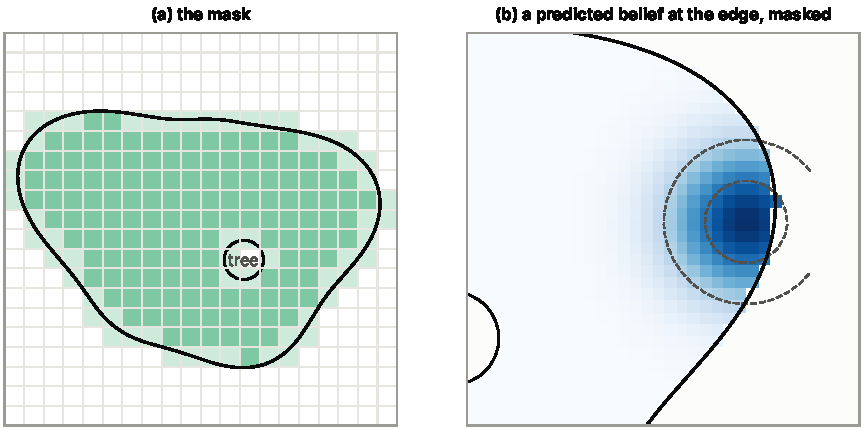
\includegraphics[width=\linewidth]{figures/ch02_potato.pdf}
\caption{A potato-shaped lawn with a tree. Left: the mask on a grid of
16-unit cells (the filter uses 4-unit cells): cells entirely on the lawn
(dark), cells cut by the edge or by the tree (light), the others (white).
Right: a predicted belief next to the edge, with 4-unit cells. The dashed
circles are the levels of the Gaussian blur; the $27\%$ of it that falls
off the lawn is set to zero, and the rest is renormalised.}
\label{fig:potato}
\end{figure}

\begin{mower}
\textbf{Boundary wire or geofence.} A \emph{boundary wire} is buried
along the edge, and the mower senses it directly: it turns back when it
reaches the wire, whatever it believes about its position. A
\emph{geofence} is a virtual boundary in software: the edge is recorded
once, by walking or driving around the lawn with the RTK GPS, and the
controller stops the robot, or turns it back, when its position comes
too close to that edge. The same recorded edge then serves twice: as the
geofence for the controller and as the mask for the filter. But a
geofence is enforced with the \emph{estimated} position, so it is only
as good as the localisation. With an RTK fix the position is good to a
few centimetres and the geofence is as good as a wall. Under trees, next
to the house, or when the correction link drops, the fix degrades and
the error can grow to metres: the robot could cross the real edge while
it believes it is inside. So the controller keeps a margin from the edge
that grows with the uncertainty of the filter (a few of its standard
deviations), or stops when the fix is lost. The assumption of the mask,
``the robot never leaves the lawn'', holds for a geofenced mower only as
long as that margin is kept; a wire does not have this weakness, which is
one reason why some mowers keep one even with an RTK GPS.
\end{mower}

On a real robot this mask is the \emph{map}. Robot navigation software
stores it as an \emph{occupancy grid}, whose cells are free, occupied or
unknown, and Monte Carlo localisation gives zero weight to particles in
occupied cells; the particle filter of \cref{ch:particle} gives zero
likelihood to particles more than 5 units off the lawn. For a mower with an RTK GPS, walking once around the lawn
records its edge, and the mask follows.

\section{Two bumps}
\label{sec:twobumps}

We make the problem hard on purpose: the robot measures only
\emph{ranges}, and only to two landmarks. A range to a landmark places
the robot on a circle around it; two ranges place it on two circles, which
meet in two points (\cref{fig:mirror}). The two points are mirror images
of each other across the line through the landmarks, and no range
measurement can tell them apart.

\begin{figure}[ht]
\centering
\begin{tikzpicture}[scale=0.95,>=Stealth]
  \coordinate (A) at (0,0);
  \coordinate (B) at (4,0);
  \def\ra{2.9}\def\rb{2.3}
  % intersection: x = (ra^2 - rb^2 + d^2)/(2d), y = sqrt(ra^2 - x^2)
  \pgfmathsetmacro{\xi}{(\ra*\ra-\rb*\rb+16)/8}
  \pgfmathsetmacro{\yi}{sqrt(\ra*\ra-\xi*\xi)}
  \draw[dashed,black!45] (-3.4,0) -- (7.0,0) node[right,black!60]
    {\small axis of $\sigma$};
  \draw[orange!85!black,thick] (A) circle (\ra);
  \draw[orange!85!black,thick] (B) circle (\rb);
  \node[star,star points=5,fill=black!70,inner sep=1.6pt] at (A) {};
  \node[star,star points=5,fill=black!70,inner sep=1.6pt] at (B) {};
  \node[below left] at (A) {$\bell_1$};
  \node[below right] at (B) {$\bell_2$};
  \draw[black!60] (A) -- (\xi,\yi) node[pos=0.5,above left] {$r_1$};
  \draw[black!60] (B) -- (\xi,\yi) node[pos=0.5,above right] {$r_2$};
  \fill[green!50!black] (\xi,\yi) circle (2.6pt)
    node[above=3pt,black] {$\p$};
  \fill[green!50!black] (\xi,-\yi) circle (2.6pt)
    node[below=3pt,black] {$\sigma(\p)$};
  \draw[<->,densely dotted,black!60] (\xi,\yi-0.15) -- (\xi,-\yi+0.15);
\end{tikzpicture}
\caption{Two ranges $r_1$, $r_2$ to two landmarks define two circles,
which meet at $\p$ and at its mirror image $\sigma(\p)$ across the line
through the landmarks. The two points have exactly the same ranges.}
\label{fig:mirror}
\end{figure}

\begin{proposition}{Mirror ambiguity}{mirror}
Let $\sigma$ be the reflection across the line through $\bell_1$ and
$\bell_2$. Then $\norm{\bell_j-\sigma(\p)}=\norm{\bell_j-\p}$ for $j=1,2$
and every $\p$. Consequently, if the belief before a range-only update is
\emph{invariant under $\sigma$}, meaning that it has the same value at
$\p$ and at $\sigma(\p)$ for every $\p$, the belief after the update is
also invariant under $\sigma$.
\end{proposition}

\begin{proof}
A reflection is an isometry, and it fixes every point of its axis, in
particular $\bell_1$ and $\bell_2$. So
$\norm{\bell_j-\sigma(\p)}=\norm{\sigma(\bell_j)-\sigma(\p)}=
\norm{\bell_j-\p}$. The likelihood of two ranges depends on the position
only through its two distances to the landmarks, so it is the same at
$\p$ and $\sigma(\p)$. The update multiplies a $\sigma$-invariant
belief by this $\sigma$-invariant likelihood, and a product of two
functions that are each the same at $\p$ and $\sigma(\p)$ is again the
same at $\p$ and $\sigma(\p)$.
\end{proof}

\begin{figure}[ht]
\centering
\begin{tikzpicture}[scale=1.0,>=Stealth,
    lab/.style={font=\small,anchor=west,inner sep=1pt,text=black},
    lead/.style={black!35,thin}]
  \coordinate (A) at (0,0);
  \coordinate (B) at (4,0);
  \def\ra{2.9}\def\rb{2.3}\def\dx{1.0}\def\dy{1.0}
  % the robot before the step: the intersection of the old circles (as in Fig. 2.7)
  \pgfmathsetmacro{\xi}{(\ra*\ra-\rb*\rb+16)/8}
  \pgfmathsetmacro{\yi}{sqrt(\ra*\ra-\xi*\xi)}
  % the robot after the step, and its new ranges
  \pgfmathsetmacro{\xn}{\xi+\dx}
  \pgfmathsetmacro{\yn}{\yi+\dy}
  \pgfmathsetmacro{\rna}{sqrt(\xn*\xn+\yn*\yn)}
  \pgfmathsetmacro{\rnb}{sqrt((\xn-4)*(\xn-4)+\yn*\yn)}
  \begin{scope}
    \clip (-1.3,-3.3) rectangle (6.5,3.3);
    \draw[dashed,black!30] (A) circle (\ra);
    \draw[dashed,black!30] (B) circle (\rb);
    \draw[orange!85!black,thick] (A) circle (\rna);
    \draw[orange!85!black,thick] (B) circle (\rnb);
  \end{scope}
  \draw[dashed,black!45] (-1.3,0) -- (6.5,0) node[right,black!60]
    {\small axis of $\sigma$};
  \node[star,star points=5,fill=black!70,inner sep=1.6pt] at (A) {};
  \node[star,star points=5,fill=black!70,inner sep=1.6pt] at (B) {};
  \node[below left] at (A) {$\bell_1$};
  \node[below right] at (B) {$\bell_2$};
  % the robot moves by d
  \draw[->,very thick,blue!70!black] (\xi,\yi) -- (\xn,\yn)
    node[pos=0.45,above left=-1pt,font=\small] {$\vect d$};
  \fill[green!50!black] (\xi,\yi) circle (2.4pt) node[left=3pt,black] {$\p$};
  \fill[green!50!black] (\xn,\yn) circle (2.4pt);
  \draw[lead] (\xn,\yn) -- (6.8,2.9) node[lab] {robot after the step};
  % its mirror image moves by sigma(d)
  \draw[->,thick,black!55] (\xi,-\yi) -- (\xn,-\yn)
    node[pos=0.5,below left=-1pt,font=\small,black] {$\sigma(\vect d)$};
  \fill[black!55] (\xi,-\yi) circle (2.4pt) node[left=3pt,black] {$\sigma(\p)$};
  \fill[black!55] (\xn,-\yn) circle (2.4pt);
  \draw[lead] (\xn,-\yn) -- (6.8,-2.9) node[lab] {mirror image of the robot};
  % the wrong hypothesis is moved by d
  \draw[->,very thick,red!75!black] (\xi,-\yi) -- (\xi+\dx,-\yi+\dy)
    node[pos=0.55,above left=-1pt,font=\small] {$\vect d$};
  \fill[red!75!black] (\xi+\dx,-\yi+\dy) circle (2.4pt);
  \draw[lead] (\xi+\dx,-\yi+\dy) -- (6.8,-1.0) node[lab] {wrong hypothesis};
  \draw[<->,densely dotted,black!60] (\xn+0.15,-\yi+\dy-0.1) --
    (\xn+0.15,-\yn+0.1);
\end{tikzpicture}
\caption{Why motion breaks the tie, with the two landmarks of
\cref{fig:mirror}. Before the step, the ranges give two circles (dashed)
that meet at the robot $\p$ and at its mirror image $\sigma(\p)$. The
robot moves by $\vect d$ (blue). The new ranges give two new circles
(orange), which meet at the new position and at its mirror image, reached
from $\sigma(\p)$ by the mirrored displacement $\sigma(\vect d)$ (grey).
The filter knows the heading and moves every hypothesis by the same
$\vect d$, also the one at $\sigma(\p)$ (red). That wrong hypothesis is
not at an intersection of the new circles (dotted gap): its ranges no
longer agree with the measurements.}
\label{fig:mirrormotion}
\end{figure}

What can tell the two points apart is the \emph{motion}, and the
likelihood then does the work. Look at one cycle of the filter, starting
from a belief with two mirror bumps.

\emph{Prediction: the motion breaks the symmetry.} The heading is known,
so the filter moves the whole belief, both bumps, by the same
displacement $\vect d$. The robot moves by $\vect d$, but its mirror
image moves by the mirrored displacement $\sigma(\vect d)$ (for a
displacement, the reflection of the vector, without translation). So the
wrong bump ends up at $\sigma(\p)+\vect d$, while the mirror image of the
robot is at $\sigma(\p)+\sigma(\vect d)$. The gap between them is
$\vect d-\sigma(\vect d)$, twice the part of $\vect d$ perpendicular to
the axis; it vanishes only when $\vect d$ is parallel to the axis. The
prediction removes no probability: it only moves the wrong bump to a
place where the ranges will not match.

\emph{Update: the likelihood removes the wrong bump.} The likelihood of
the new ranges is $\sigma$-invariant (\cref{prop:mirror}). It is large
near the two intersections of the new circles: the robot and its mirror
image (\cref{fig:mirrormotion}). The right bump sits at one of them; the
wrong bump sits away from both, because two points have the same
distances to two distinct landmarks only if they are equal or mirror
images (two circles with distinct centres meet in at most two points). So
the update multiplies the wrong bump by a smaller value than the right
one, and after renormalisation the wrong bump has lost mass to the right
one.

Neither step works alone. Without motion, or with a motion parallel to
the axis, the belief stays $\sigma$-invariant and, by
\cref{prop:mirror}, every update keeps the two bumps as they are. Without
the likelihood, the prediction only moves and blurs the bumps.

\emph{Why it takes several steps.} Write $\rho_j(\vect x)=
\norm{\bell_j-\vect x}$ for the distance from a point $\vect x$ to the
landmark $\bell_j$. The measured range is $z_j=\rho_j(\p)+v_j$, with a
noise $v_j\sim\Normal(0,\sigma_r^2)$, $\sigma_r=5$. Call $\vect w$ the
position of the wrong bump, and $e_j=\rho_j(\vect w)-\rho_j(\p)$ its
\emph{range errors}.

First, the update acts on the ratio of the two masses through the ratio
of the likelihoods. Treat each bump as if its mass were at one point: $m_{\vect w}$
at $\vect w$ and $m_{\p}$ at $\p$ before the update. The update
\eqref{eq:update} multiplies each mass by the likelihood at its point and
by the same constant $\eta$, so after the update
\[
  \frac{\eta\,p(\z\mid\vect w)\,m_{\vect w}}{\eta\,p(\z\mid\p)\,m_{\p}}
  =\frac{p(\z\mid\vect w)}{p(\z\mid\p)}\cdot\frac{m_{\vect w}}{m_{\p}} :
\]
$\eta$ cancels, and the ratio of the masses is multiplied by the ratio of
the likelihoods.

Next, that ratio. The two ranges have independent Gaussian noises, so the
likelihood at a point $\vect x$ is
$p(\z\mid\vect x)=C\prod_je^{-(z_j-\rho_j(\vect x))^2/(2\sigma_r^2)}$,
with a constant $C$ that does not depend on $\vect x$. At the robot,
$z_j-\rho_j(\p)=v_j$. At the wrong bump,
$z_j-\rho_j(\vect w)=\bigl(z_j-\rho_j(\p)\bigr)-\bigl(\rho_j(\vect w)
-\rho_j(\p)\bigr)=v_j-e_j$. Then, line by line:
\begin{align*}
  \frac{p(\z\mid\vect w)}{p(\z\mid\p)}
  &=\frac{C\prod_je^{-(v_j-e_j)^2/(2\sigma_r^2)}}
         {C\prod_je^{-v_j^2/(2\sigma_r^2)}}
  &&\text{the two likelihoods}\\
  &=\prod_j\exp\Bigl(-\frac{(v_j-e_j)^2-v_j^2}{2\sigma_r^2}\Bigr)
  &&\text{$C$ cancels; $e^a/e^b=e^{a-b}$, factor by factor}\\
  &=\prod_j\exp\Bigl(-\frac{e_j^2-2e_jv_j}{2\sigma_r^2}\Bigr)
  &&(v_j-e_j)^2=v_j^2-2e_jv_j+e_j^2\\
  &=\exp\Bigl(-\sum_j\frac{e_j^2}{2\sigma_r^2}
   +\sum_j\frac{e_jv_j}{\sigma_r^2}\Bigr)
  &&\textstyle\prod_je^{a_j}=e^{\sum_ja_j}.
\end{align*}
In the exponent, the first term always favours
the right bump, and it grows like the \emph{square} of the range errors.
The second is random: the noises $v_j$ are independent, with mean $0$
and variance $\sigma_r^2$, so it has the mean $0$ and the variance
$\sum_je_j^2\sigma_r^2/\sigma_r^4=\sum_je_j^2/\sigma_r^2$, that is the
standard deviation $\sqrt{\sum_je_j^2}/\sigma_r$: it grows only like the
errors themselves.
While the range errors are smaller than $\sigma_r$, both terms are small,
and the second can favour either bump. Once they are larger than
$\sigma_r$, the first term wins, and the wrong bump loses most of its mass
at every update. The range errors grow with the gap, so the filter needs
a few steps of driving before the ranges can separate the two bumps.

\begin{figure}[ht]
\centering
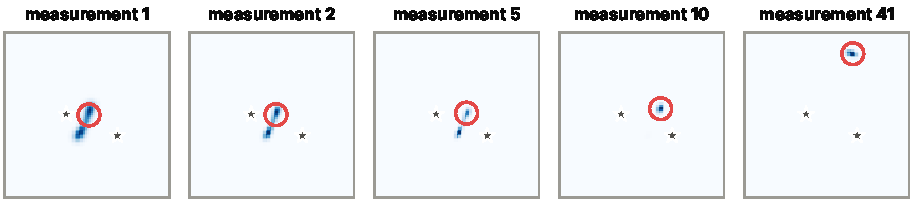
\includegraphics[width=\linewidth]{figures/ch02_grid_bimodal.pdf}
\caption{Grid belief (darker is more probable; a power-law colour scale
makes small masses visible) with range-only sensing to two landmarks
(stars); the red circle surrounds the true position. The first measurement gives a
belief symmetric about the line through the landmarks (nearly: the
uniform start is cut off by the edges of the lawn, which are not symmetric
about that line): two bumps. Both survive for a few measurements, and at
measurements 4 and 5 the \emph{wrong} one carries more mass than the right
one (at measurement 5, $0.65$ against $0.35$ on the two sides of the
line; notebook~01 prints these masses for the first ten measurements). As
the robot drives on, the wrong bump stops agreeing with the ranges: by
measurement 8 it has disappeared, and the belief then follows the robot.}
\label{fig:gridbimodal}
\end{figure}

The run of \cref{fig:gridbimodal} has only the first two landmarks
(seed 1) and starts from a uniform belief over the lawn. The table
follows the \emph{wrong track}: the mirror image of the robot at
measurement 1, moved afterwards by the robot's own displacements. For
each measurement $k$ it gives the gap to the mirror image of the robot,
the range errors $e_1,e_2$ of the wrong track, the range noises
$v_1,v_2$, the factor by which the update multiplied the ratio (mass on
the wrong side)\,/\,(mass on the right side) of the grid, and the mass on
the wrong side after the update (notebook~01 prints all of them).
\begin{center}
\small
\begin{tabular}{@{}rrrrrrrr@{}}
\toprule
$k$ & gap & $e_1$ & $e_2$ & $v_1$ & $v_2$ & update factor &
mass on the wrong side\\
\midrule
 1 &  0.0 &   0.0 &   0.0 &  1.7 &  4.5 & ---  & 0.50\\
 2 &  4.3 &  $-$1.4 &  $-$1.0 &  2.7 & $-$0.8 & 1.09 & 0.51\\
 3 &  8.5 &  $-$2.7 &  $-$2.2 &  0.0 &  6.5 & 0.80 & 0.44\\
 4 & 13.2 &  $-$3.9 &  $-$3.5 &  1.1 & $-$5.6 & 1.70 & 0.57\\
 5 & 18.0 &  $-$5.0 &  $-$5.0 &  0.8 & $-$6.1 & 1.44 & 0.65\\
 6 & 23.5 &  $-$6.2 &  $-$6.8 & $-$2.5 &  4.5 & 0.35 & 0.39\\
 7 & 29.6 &  $-$7.4 &  $-$8.9 &  4.6 & $-$6.2 & 0.45 & 0.22\\
 8 & 35.0 &  $-$8.3 & $-$10.8 & $-$2.3 &  3.8 & 0.06 & 0.01\\
 9 & 40.9 &  $-$9.3 & $-$12.9 &  1.3 & $-$1.7 & 0.05 & 0.00\\
10 & 47.5 & $-$10.4 & $-$15.2 & $-$6.0 &  3.4 & 0.02 & 0.00\\
\bottomrule
\end{tabular}
\end{center}
Three phases appear.
\begin{itemize}[nosep]
  \item \emph{Measurement 1.} The first update turns the uniform belief
        into two mirror bumps, with half of the mass each.
  \item \emph{Measurements 2 to 5.} The gap grows by about $4$ to $5$
        units per step, but the range errors stay at or below
        $\sigma_r=5$, so the update factors are close to $1$ and the
        noise decides their direction. At measurements 4 and 5 it
        favours the wrong bump: the measured range to $\bell_2$ was short
        by $5.6$ and $6.1$, and the wrong track is also closer to
        $\bell_2$ than the robot ($e_2=-3.5$ and $-5.0$), so its ranges
        fit the measurements better. The wrong side then carries $0.65$ of
        the mass.
  \item \emph{Measurements 6 to 10.} The range errors exceed $\sigma_r$,
        the first term wins, and the factors drop to $0.35$, $0.45$,
        then about $0.05$ and below: the wrong bump is gone by
        measurement 8.
\end{itemize}
For the bumps as a whole the factors are not exactly the ratio of the
likelihoods at two points, because each bump is spread over many cells,
but they follow the same pattern.

\begin{inwords}
The true posterior can have several separate bumps, and the right bump
need not be the biggest one for a while. A filter that represents only
one bump, or that commits early to the most probable one, could have
chosen the mirror image at measurement 4 or 5, with no way back. A Gaussian
belief is worse still: its mean would sit \emph{between} the two bumps,
where the robot certainly is not.
\end{inwords}

\section{The cost of a grid}

The grid is exact up to discretisation and can represent any belief. Its
cost is the number of cells, and every step touches every cell. If the
state has $d$ coordinates and each is cut into $n$ intervals, the grid has
$n^d$ cells. With $n=80$: $6\,400$ cells for the position, about half a million for the
pose $(x,y,\theta)$ (the classic \emph{Markov localisation} of the 1990s,
feasible), $2.6\times10^{11}$ for a pose with its three velocities (six
dimensions). And at any
time, almost all of those cells have negligible probability. There are two
ways out, and the rest of the book follows both:
\begin{enumerate}[nosep]
\item \emph{assume a shape} for the belief, a Gaussian described by a mean
  and a covariance ($d+d(d+1)/2$ numbers): the Kalman family,
  Part~II;
\item \emph{sample} the belief, putting the computation only where the
  probability is: the particle filter, Chapter~\ref{ch:particle}.
\end{enumerate}

\begin{practice}[\nb{01\_bayes\_filter.ipynb}, \code{grid.py}]
\code{GridFilter} implements the predict and update steps above on cells
4 units wide ($80\times80$ cells), with \code{sensor="range"} or \code{"range\_bearing"}. The notebook
reproduces \cref{fig:gridbimodal} and compares the grid filter with dead
reckoning: with two noisy ranges per step, its median error after step 20
is $2.3$, less than half the range noise $\sigma_r=5$, although the cells are
4~units wide. Things to try:
switch to range--bearing (a bearing tells the side of the axis and the
ambiguity disappears), use all four landmarks, or enlarge the cells.
\end{practice}

\begin{mower}
A mower that wakes up in the morning does not know where it was left. The
first measurements are rarely enough to pin it down, especially with
symmetric landmark layouts (four beacons at the corners of a rectangular
lawn are symmetric under a half-turn) or with only ranges, as with radio
beacons. The ambiguity is real, and a localisation system must be able to
carry several hypotheses until the motion resolves them.
\end{mower}

\section*{What to remember from this chapter}
\addcontentsline{toc}{section}{What to remember}

\begin{enumerate}[nosep]
  \item The belief $\bel(\x_t)$ is the distribution of the current pose
    given all controls and measurements so far. It is the complete answer
    to ``where is the robot?''.
  \item The Bayes filter updates it in two steps. \emph{Predict}
    \eqref{eq:predict}: push the belief through the motion model; it
    blurs. \emph{Update} \eqref{eq:update}: multiply by the likelihood of
    the new measurement and renormalise; it sharpens.
  \item The normaliser $\eta^{-1}$ is the value of the density that the
    filter gave to the measurement before seeing it: a measure of
    surprise.
  \item The exact belief can have several bumps, and the right one is not
    always the biggest.
  \item A grid computes the recursion with no assumption on the shape of
    the belief, but its cost grows exponentially with the dimension of the
    state. Every other filter of the book is a cheaper approximation of
    the same recursion.
\end{enumerate}

\FloatBarrier
\section*{Exercises}
\addcontentsline{toc}{section}{Exercises}

\begin{enumerate}[label=\textbf{2.\arabic*},ref=2.\arabic*]
\item\label{ex:twostate} \emph{A two-state filter.} In the setting of
  \cref{ex:grassgravel}, start from $\bel=(0.5,0.5)$ and compute the belief
  after the readings ``rough'', ``rough''.
\item\label{ex:blur} Show that blurring with $\Normal(\vect0,\Sigma_1)$ and
  then with $\Normal(\vect0,\Sigma_2)$ is the same as blurring once with
  $\Normal(\vect0,\Sigma_1+\Sigma_2)$. What does it say about the width of
  a grid belief after $t$ predictions without updates?
\item\label{ex:nomotion} Suppose the robot is parked (so the prediction is
  the identity) and keeps receiving range-only readings from the same two
  landmarks. Show that the belief stays bimodal forever, and that each bump
  keeps probability $1/2$ if the prior was symmetric.
\item\label{ex:gridcost} A robot localises on a $30\times30$\,m lawn with a
  pose grid of $5$\,cm and $1^\circ$. How many cells is that, and how many
  bytes in single precision? How many floating-point operations does one
  prediction cost if it is done as a full sum over pairs of cells?
\item\label{ex:potato} \emph{A potato-shaped lawn.} The lawn of
  \cref{fig:potato} has a curved edge and a tree.
  \begin{enumerate}[nosep]
    \item Show that setting the belief of the cells off the lawn to zero
          and renormalising is Bayes' rule for an observation ``the
          robot is on the lawn''. What is its likelihood?
    \item Why is the convolution of \cref{prop:conv} still the exact
          prediction far from the edge, but not next to it? What does the
          masking assume about the robot?
    \item The lawn fits in a $320\times320$ square. With 4-unit cells,
          $2749$ of the $6400$ cells of the square have their centre on
          the lawn. How can the filter avoid storing and updating the
          others?
  \end{enumerate}
\end{enumerate}

\subsection*{Solutions}

\solution{2.1} Each step is a prediction followed by an update, as in
\cref{ex:grassgravel}: the robot may change surface between two readings.
Order the states as $(G,P)$; the sensor says ``rough'' with probability
$0.3$ on the grass and $0.8$ on the path.

\emph{First step.} Predict: $\belbar(G)=0.9\times0.5+0.1\times0.5=0.5$,
and likewise $\belbar(P)=0.5$. The belief $(0.5,0.5)$ does not change: as
much probability flows from the grass to the path as back. Update with
``rough'': multiply each predicted probability by the probability of the
reading in that state, add, and divide by the sum.
\begin{center}
\begin{tabular}{lccc}
  \toprule
  & predicted & $\times\,p(\text{rough}\mid\cdot)$ & new belief\\
  \midrule
  grass & $0.5$ & $0.5\times0.3=0.15$ & $0.15/0.55=0.273$\\
  path  & $0.5$ & $0.5\times0.8=0.40$ & $0.40/0.55=0.727$\\
  \midrule
  total & $1$ & $0.55$ & $1$\\
  \bottomrule
\end{tabular}
\end{center}
The sum $0.55$ is the probability that the filter gave to the reading
``rough'' before seeing it.

\emph{Second step.} Predict: the robot is on the grass if it was there and
stayed, or on the path and left it:
\[
  \belbar(G)=0.9\times0.273+0.1\times0.727=0.318,\qquad
  \belbar(P)=0.1\times0.273+0.9\times0.727=0.682 .
\]
Update with ``rough'':
\begin{center}
\begin{tabular}{lccc}
  \toprule
  & predicted & $\times\,p(\text{rough}\mid\cdot)$ & new belief\\
  \midrule
  grass & $0.318$ & $0.318\times0.3=0.0955$ & $0.0955/0.641=0.149$\\
  path  & $0.682$ & $0.682\times0.8=0.5455$ & $0.5455/0.641=0.851$\\
  \midrule
  total & $1$ & $0.641$ & $1$\\
  \bottomrule
\end{tabular}
\end{center}
The belief after the two readings is $(0.149,\,0.851)$.

\emph{What the prediction did.} Without the prediction between the two
readings, that is if the robot could not change surface, the two readings
would multiply $(0.5,0.5)$ by $0.3\times0.3=0.09$ and $0.8\times0.8=0.64$,
which gives $(0.09,0.64)/0.73=(0.123,\,0.877)$. The filter is less sure
of the path, $0.851$ instead of $0.877$: between the readings, the
prediction moved $0.1\times0.727=0.073$ of probability from the path to
the grass, and only $0.1\times0.273=0.027$ back. A reading taken
\emph{before} a possible change of surface says less about the surface
\emph{after} it.

\solution{2.2} The idea: blurring a density with a Gaussian is adding an
independent Gaussian noise to a random vector that has this density, and
two independent Gaussian noises add up to one.

\emph{Step 1: a blur is an added noise.} Let $X$ have the density $b$, and
let $X_1\sim\Normal(\vect0,\Sigma_1)$ be independent of $X$, with the
density $g_1$. By the probabilistic meaning of the convolution
(\cref{sec:grid}), $b\ast g_1$ is the density of $X+X_1$.

\emph{Step 2: the second blur.} Let $X_2\sim\Normal(\vect0,\Sigma_2)$,
with the density $g_2$, be independent of $(X,X_1)$, hence of $X+X_1$. By
the same result, $(b\ast g_1)\ast g_2$ is the density of $(X+X_1)+X_2$.

\emph{Step 3: the two noises are one.} Group the terms the other way:
$(X+X_1)+X_2=X+(X_1+X_2)$. The sum $X_1+X_2$ is Gaussian, as a sum of two
independent Gaussians (\cref{lem:affine}, in \cref{ch:kalman}); its mean
is $\vect0$, and its covariance is $\Sigma_1+\Sigma_2$, because the
covariances of independent vectors add (\cref{sec:grid}). It is
independent of $X$, since $X_1$ and $X_2$ are. So, by Step~1 again, the
density of $X+(X_1+X_2)$ is $b\ast g_{12}$, with $g_{12}$ the density of
$\Normal(\vect0,\Sigma_1+\Sigma_2)$.

\emph{Conclusion.} Steps 2 and 3 give the density of the same random
vector, so $(b\ast g_1)\ast g_2=b\ast g_{12}$: two blurs are one blur with
the summed covariance.

\emph{After $t$ predictions without update.} Each prediction shifts the
belief and blurs it with $\Normal(\vect0,\Sigma)$ (\cref{prop:conv}). The
shifts only move the belief. Applying the result $t-1$ times, the $t$
blurs are one blur with $\Normal(\vect0,t\Sigma)$. Along a direction
$\vect u$, the standard deviation of that blur is
$\sqrt{t\,\vect u\T\Sigma\vect u}=\sqrt t\,\sqrt{\vect u\T\Sigma\vect u}$:
the width of the belief grows like $\sqrt t$. On the grid of
\cref{sec:grid}, each blur has the standard deviation $1.2$ units (the
floor of $0.3$ cell, notebook~01), so after $t$ predictions the blur alone
has the standard deviation $1.2\sqrt t$: for example $12$ units, three
cells, after $100$ predictions. This assumes a known heading, as in
\cref{prop:conv}. When the heading itself is uncertain, its errors
accumulate and turn into sideways errors that grow faster: on a straight
path the variance of the lateral error grows like $t^3$
(\cref{prop:deadreckoning}), so its standard deviation grows like
$t^{3/2}$.

\solution{2.3} There are two claims: the two bumps keep equal masses, and
the belief stays made of two bumps, which become narrower.

\emph{The belief after $k$ readings.} The prediction is the identity, so
each step only multiplies the belief by the likelihood of the new
readings $\z_i$ and renormalises. After $k$ steps, collecting the
constants into one,
\[
  \bel_k(\p)=\eta\,\bel_0(\p)\prod_{i=1}^kp(\z_i\mid\p).
\]

\emph{Equal masses.} By \cref{prop:mirror}, each likelihood is
$\sigma$-invariant: $p(\z_i\mid\sigma(\p))=p(\z_i\mid\p)$. If the prior is
$\sigma$-invariant too, every factor of the product takes the same value
at $\p$ and at $\sigma(\p)$, so $\bel_k(\sigma(\p))=\bel_k(\p)$ for every
$k$. The reflection maps the half-plane on one side of the axis onto the
other half-plane and keeps areas, so the two half-planes have the same
mass. The axis itself has zero area, so each half-plane has the mass
$1/2$, exactly, at every step, not only in the limit. If the prior is not
symmetric, the same argument shows that the ratio
$\bel_k(\sigma(\p))/\bel_k(\p)=\bel_0(\sigma(\p))/\bel_0(\p)$ never
changes: the readings cannot correct an asymmetry of the prior either.

\emph{Two narrowing bumps.} Take one landmark $\bell$, at the distance
$\rho(\p)=\norm{\bell-\p}$ from $\p$, and its $k$ readings
$r_1,\dots,r_k$, with independent noises $\Normal(0,\sigma_r^2)$. Write
$\bar r=\frac1k\sum_ir_i$ for their mean. The product of their
likelihoods is
\[
  \prod_{i=1}^ke^{-(r_i-\rho(\p))^2/(2\sigma_r^2)}
  =\exp\Bigl(-\frac{1}{2\sigma_r^2}\sum_{i=1}^k\bigl(r_i-\rho(\p)\bigr)^2\Bigr).
\]
Write $r_i-\rho=(r_i-\bar r)+(\bar r-\rho)$ and expand the square:
\[
  \sum_i(r_i-\rho)^2
  =\sum_i(r_i-\bar r)^2+2(\bar r-\rho)\sum_i(r_i-\bar r)+k(\bar r-\rho)^2
  =\sum_i(r_i-\bar r)^2+k(\bar r-\rho)^2 ,
\]
because $\sum_i(r_i-\bar r)=\sum_ir_i-k\bar r=0$. The first sum does not
contain $\p$, so
\[
  \prod_{i=1}^ke^{-(r_i-\rho(\p))^2/(2\sigma_r^2)}
  =C\,\exp\Bigl(-\frac{(\bar r-\rho(\p))^2}{2\,\sigma_r^2/k}\Bigr),
\]
with a constant $C$. This is the likelihood of a single reading $\bar r$
with the standard deviation $\sigma_r/\sqrt k$. The positions that agree
with the readings of this landmark form a ring around it, of radius about
$\bar r$ and width proportional to $\sigma_r/\sqrt k$. The two rings, one
per landmark, meet in two spots around $\p$ and $\sigma(\p)$, which shrink
like $1/\sqrt k$. Only a motion that is not parallel to the axis, or a
third landmark off the axis, can break the tie (\cref{sec:twobumps}).

\solution{2.4} \emph{Cells.} Along each side, $30\,\text{m}/5\,\text{cm}
=600$ cells; for the heading, $360$ cells of $1^\circ$. In total
$600\times600\times360=129\,600\,000\approx1.3\times10^8$ cells.

\emph{Memory.} In single precision a number takes $4$ bytes, so the
belief takes $4\times1.3\times10^8\approx5.2\times10^8$ bytes, about
$520$\,MB.

\emph{A prediction as a full sum.} Write the prediction
\eqref{eq:predict} on the cells as $\bar b_i=\sum_jT_{ij}b_j$, with
$T_{ij}$ the probability of going from the cell $j$ to the cell $i$. Each
of the $n\approx1.3\times10^8$ new values is a sum of $n$ products, so the
prediction costs $n^2\approx1.7\times10^{16}$ multiplications and as many
additions. At $10^{10}$ operations per second, a fast processor, that is
$3.4\times10^6$ seconds, about $39$ days, for one prediction. The matrix
$T$ itself, with $n^2$ entries, would not fit in any memory.

\emph{Using the structure.} The probability of going from $j$ to $i$ is
negligible unless $i$ is near the cell reached from $j$ by the commanded
motion: the prediction is a shift and a local blur (\cref{prop:conv}).
A Gaussian blur over $5$ cells along each of the three axes, done one
axis at a time, costs $3\times5=15$ multiplications per cell, about
$2\times10^9$ per prediction: a fraction of a second. So the grid filters
that work in practice are built on such shifts and blurs, or on sparse
transitions. Even then, $520$\,MB of belief updated several times per
second is a lot for an embedded computer.

\solution{2.5}
\begin{enumerate}[nosep]
  \item Let $L$ be the set of the lawn cells, and take as observation
        the statement ``the robot is on the lawn''. Its likelihood in the
        cell $C_i$ is the probability of that statement when the robot
        is in $C_i$: $1$ if $i\in L$ and $0$ otherwise. Bayes' rule
        \eqref{eq:update} on the grid multiplies each predicted
        probability by the likelihood and divides by the sum:
        \[
          b_i=\frac{\mathbf 1_L(i)\,\bar b_i}{\sum_j\mathbf 1_L(j)\,\bar b_j}
          =\begin{cases}\bar b_i/\sum_{j\in L}\bar b_j,&i\in L,\\
          0,&i\notin L.\end{cases}
        \]
        That is the mask: the cells off the lawn get $0$, and the others
        are renormalised. The sum $\sum_{j\in L}\bar b_j$ is the
        probability that the prediction gave to the lawn, like the
        $0.43$ of \cref{ex:grassgravel}; in \cref{fig:potato}, $27\%$
        falls off the lawn, so it is $0.73$.
  \item The convolution moves every bit of probability by the commanded
        displacement and spreads it by the noise, whatever is around: it
        describes a robot that moves as if there were no edge. Far from
        the edge, the blur only reaches cells on the lawn, nothing is
        removed, and the convolution is the whole prediction. Next to the
        edge, the blur reaches cells off the lawn, where the robot cannot
        be, and the mask removes that probability. Masking is then exact
        under one assumption: the robot moves as if there were no edge,
        and we learn afterwards that it is still on the lawn, as in~(a).
        A real mower does not move like that near the edge: its boundary
        wire or its geofence stops it or turns it back. So the masking is
        an approximation, good when little of the belief lies within a
        few standard deviations of the blur from the edge.
  \item Store only the $2749$ lawn cells, for example as a list of the
        cell indices with their probabilities, or as a sparse array. The
        prediction computes the blur only at these cells, from their
        neighbours on the lawn, and the update only touches them. That is
        $2749/6400=43\%$ of the square, in memory and in time. When the
        cells are small compared with the lawn, a \emph{quadtree}, with
        small cells along the edge and large ones elsewhere, saves more:
        its number of cells grows like the length of the edge divided by
        the side of the smallest cells, not like the area divided by the
        square of that side (\cref{app:quadtree}).
\end{enumerate}
